\chapter{Objective}
\begin{comment}
The objective of the work is composed by the goals the software have to reach and the definition of the requirements for achieving them. These two aspects are described in the following sections.
\end{comment}

	\section{The Goals of the Software}
	The software to be designed and developed is a visual module for the cognitive architecture ACT-R, whose aim is to improve ACT-R visual perception in order to make it more similar to the human one. 
	
	After a model is developed in ACT-R, it needs to be validated. Model validations usually are realized with experiments in which human beings take part. For every experiment a specific program is created in order to measure some variables as, for example, the time needed to complete a task and the accuracy of the result. The parameters obtained by the model are then compared with the ones obtained in these experiments.
 
	Image~\ref{fig:RushHourHuman} shows a test case of an experiment in which the goal is to solve some levels of the game \emph{Rush Hour}. As shown, the grid contains some colored rectangles, each of which represents a car. The player must free the red one making it go out of the grid through the exit on the right. The cars can be moved only in the horizontal and vertical directions. The goal of the game is to free the red car in the minimum number of moves and in the shortest possible time.

	\begin{figure}[!h]
	  \begin{center} 
	    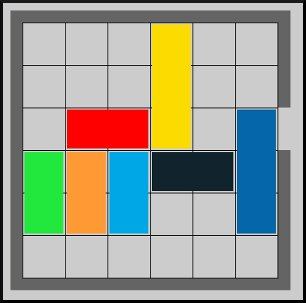
\includegraphics[scale=0.6]{images/ch_03/originale.jpg}	
	  \end{center} 
	  \caption{\textit{Example of level of Rush Hour game}}
	  \label{fig:RushHourHuman}	
  	\end{figure}
	
	For each test of the experiment, the ad-hoc program shows the image with the initial configuration and the person has to give the solution of the game by clicking on the rectangles in the order he thinks to be the correct one and the best one to free the red car. As the program never updates the image, the player has to remember the moves he makes. The software manages to interpret the direction of the shift by analyzing the movement of the eye, thanks to a module of \emph{eye tracking}. Moreover, it records the movements of the mouse, the clicks of the mouse, the time needed to give the solution and the correctness of the solution. 

	The models written in ACT-R that need to process images, like the one used to solve the rush hour game, at the moment skip the image processing step and start directly from a list of objects which is written directly in the input of the model. ACT-R can not accomplish this task because its visual module does not provide functions for the image processing.
	This fact represents a big limitation for the architecture and leads to a significant gap between the human cognitive system and the framework one. In addition, writing the objects in a model leads to other problems as, for example, the loss of time to write the object for every single test, the consequent delay of the work and the non-scalability of this approach.
	
	The goal of the developed software is to reduce the gap between the human and ACT-R visual systems, being a starting point for a complete \todo{and general purpose??} tool for the cognitive architecture to recognize objects. To achieve this, the software analyzes the image created for the user, processes it extracting the features needed by ACT-R and stores the information in dedicated data structures. Then, when requested by the cognitive architecture, it communicates to the artificial intelligent framework all the stored information. 
	

\begin{comment}
	The goals of the software  are to simplify the psychologists work of defining new test cases for experiments in ACT-R and to recognize objects during the navigation of robots.

	At the moment, a psychologist, in order to insert a new test in ACT-R, has to create two interfaces, one for the user and one for ACT-R.
	The interface for the user is generally an image and can be created with any graphical editor. 
	The interface for ACT-R, instead, is much more complicated and requires the creator of the experiment to write each shape directly on the visual buffer. \todo{check correctness of this} \todo{check if the visual buffer has been introduced}
	
	The following picture shows an example of the two images used in the test.
	The one on the left is the image shown to the user while the image on the right represents the ACT-R one. 
		
	\begin{figure}[h]
	  \begin{center} 
	    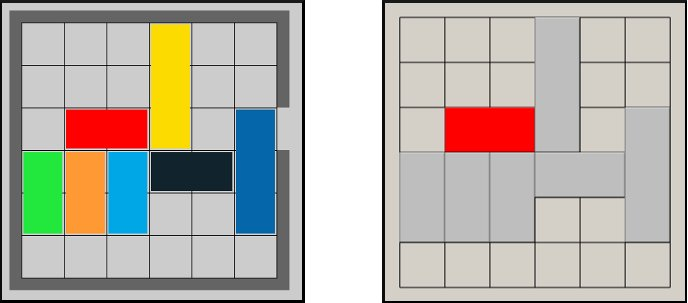
\includegraphics[scale=0.6]{images/ch_03/original_and_visicon.jpg}
	  \end{center} 
	  \caption{\textit{The two versions of the image: on the left the image for the use, on the right the image shown in ACT-R}}  
	  \label{fig:OriginalAndVisiconImages}
  	\end{figure}

	

	So, to create a test, the psychologist has to create the same image in two different formats.
	This double work causes a loss of time for the psychologist. Moreover, writing by hand all the shapes on ACT-R visual buffer is a low-level activity and can lead to stress and consequently to errors.


	The purpose of the software is to avoid to the psychologists the activity of writing on ACT-R visual buffer. To achieve this, the software analyzes the image created for the user, processes it extracting the features needed by ACT-R and communicates them to the artificial intelligence framework, which designs them automatically on its visual buffer. 
	This relieves the creators of the test of the double task described above leading to a better working experience, a less stressed work and a lower probability of errors.
	

	\todo{will i put this? or will i put it in the future developments? at the beginning it was a requirement. Will i say that the object recognition part is not developed yet?}
\end{comment}


	\section{Requirements}
	The requirements are grouped in the following sections according to the functional/non-functional classification. 
	%The simple shapes recognized are circles, triangles, squares, rectangles and ellipses.
	%Another important feature that must be introduced is the recognition of the text

		\subsection{Functional Requirements}
		The objective of the work is to design and implement a standalone software module which receives as input an image and is able to analyze it and extract some features of it.

		The input image is a color image which contains simple shapes. The shapes must not be overlapping and must have the same color hue.

		The software must recognize simple shapes, in particular:
		\begin{itemize}
	    		\item triangles;
			\item rectangles;
			\item quadrilaterals;
			\item circles.
		\end{itemize}

		For each shape, it must calculate:
		\begin{itemize}
		    	\item area;
		    	\item perimeter;
			\item dimensions;
			\item rotation;
			\item a rectangular bounding box;
			\item center;
		\end{itemize}

		Moreover, the software has to:
		\begin{itemize}
			\item recognize the color of a single pixel;
			\item recognize the color of a shape;
		    	\item calculate distances between objects;			
			\item make dimensional comparisons between objects;
			\item calculate the relative position of one object in respect with another one.
		\end{itemize}

\begin{comment}
		The shapes to be recognized are circles, triangles, rectangles and squares. 
		The color of the object is calculated averaging all the pixels of the object.
		The rotation is defined as the angle between the less sloped segment of the boundary of the object and the horizontal direction, calculated in the counterclockwise order.
		The bounding box is a rectangle whose coordinates are calculated getting the minimum and the maximum coordinates in the horizontal and vertical directions of the pixel of the image. 
		The center of a shape is the center of the bounding box.
		The distances between objects are calculated in two different ways. The first one is the distance between the centers of two shapes. The second one is the minimum distance calculated between each vertex of the bounding box of the first shape and all the vertexes of the bounding box of the second shape.
		The dimensional relation between two objects is made comparing their areas. 
		The relative position of two objects is found comparing the positions of the two top-left vertexes of each bounding box.
\end{comment}

		The software must be able to communicate with ACT-R. 
		In particular, ACT-R must signal to it which is the image to process and ask for a the features to be extracted. The module must return all the information extracted by ACT-R.

		\subsection{Non-Functional Requirements}
		The non-functional requirements described in the following subsections are respectively the requirements on the product and the organizational ones.

			\subsubsection{Product Requirements}
			The software module must be multi-purpose, portable and must work in background.
			As multi-purpose is intended that, if possible, it should be easily adapted to be able to work with all the experiments that will be put in place in the future. Moreover, there should be the possibility to adapt the software in order to use it as a shape recognition tool in the navigation with robots. For this topic, see~\ref{futureDev}. 
			As portability is intended that it has to work on more operative systems.
	
			\subsubsection{Organizational Requirements}
			The language of the implementation of the software must be C++. 
			The computer vision library to be used must be OpenCV.
			The adopted version control system must be Git.
			A strict monitoring of the work is required.

	\section{Future Development}\label{futureDev}
		Another scope in which the software will be used is the robot navigation. 
		The shapes identified by the software will be used like a starting point for an object recognition process. 
		The information about these objects, then, will be used by ACT-R in order to take intelligent decisions during the robot navigation inside a building, without any other knowledge of the environment. 
		The object recognition module has not been developed yet nor the requirements for achieving this second goal are defined. 	

		Moreover, in order to scale with other kinds of experiments an \emph{optical character recognition} tool will be added and other simple shapes will be recognized.



\begin{comment}
	\section{Functional Requirements}
		The objective of this work is to make easier the creation of an ACT-R test.\newline
		At the moment, a psychologist, in order to create a test, has to create two interfaces, one for the user and one for ACT-R. The user interface is quite simple, it is formed by simple shapes that can have different colours and words. The user has to read or watch the screen and then choose between a series of possibilities. In order to be analysed by ACT-R, this interface must have a corresponding one, which is simpler and contains only the most important features of the first one. This "simpler" interface is given as input to ACT-R and is written according to a fixed pattern. The figure below shows an example of the user interface of a test and of its corresponding one.\newline \newline	

			%qui metterei le due figure


		The purpose of this work is to create a module which is able to receive as input the user interface, recognize the main features in it and create the corresponding ACT-R interface, which must contain only such features. In order to do this, the software must be made by two parts. The first part will analyze the image. It will recognize and distinguish simple shapes, such as squares, rectangles, circles, stars, arrows; distinguish the colours of the objects; determine the position of each object in the image and recognize the text in the image. The second part will create the correspondent interface for ACT-R, thus... \newline \newline	 %% come deve fare a creare lquestai nterfaccia (lisp o qualcos altro)???? 
		  
		The software is going to be tested with several ACT-R test.
	
	\section{Non Functional Requirements}
\end{comment}	

